%% SECTION HEADER /////////////////////////////////////////////////////////////////////////////////////
\section{Model-assisted severity damage assessment }
\label{sec:madif}

%% SECTION CONTENT ////////////////////////////////////////////////////////////////////////////////////

%% SUBSECTION HEADER //////////////////////////////////////////////////////////////////////////////////
The process of determining the damage size is shown in the flowchart in Fig. \ref{fig:Flowchart}.
Before inspecting a given \ac{hsc} panel, a numerical analysis is performed to determine a function that describes the effect of damage on wave propagation.
Then the model is subjected to experimental validation.
If the simulation results do not agree with the measured results, the material parameters of the components should be adjusted.
In the dissertation, the volume fraction fibre of the \ac{cfrp} is adjusted to determine a wave velocity \cite{kudela2007modelling} and a damping coefficient of the skin to set the magnitude of the registered signals \cite{wandowski2017guided}.
\begin{figure}[H]
	\begin{center}
		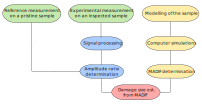
\includegraphics[width=0.95\textwidth]{Chapter_3/flowchart}
	\end{center}
	\caption{A flowchart representing the process for damage size estimation.}
	\label{fig:Flowchart}
\end{figure}

When the structure model is developed, several computer simulations for various damage sizes must be conducted to determine the \ac{madif}, a cornerstone of the dissertation. This function determines the severity of the \ac{hsc} damage based on the signal received by the sensor.
Several excitation signals and damage indices will be considered to select the best \ac{madif}.
The selection criterion will be the monotonicity and the function slope over the considered range of the damage size. Then, the damage magnitude is obtained from the \ac{madif} for the measured signal and normalised to the reference one.


